\documentclass[oneside,12pt]{book}
\usepackage[letterpaper]{geometry}
\usepackage{amsmath,amsthm,amssymb}
\usepackage{scalerel}
\usepackage{mathpazo}
\usepackage{esint}

% custom script-r
\renewcommand{\b}{\mathbf}
\newcommand{\h}[1]{\mathbf{\hat{#1}}}
\def\r{{\mbox{$\resizebox{.09in}{.08in}{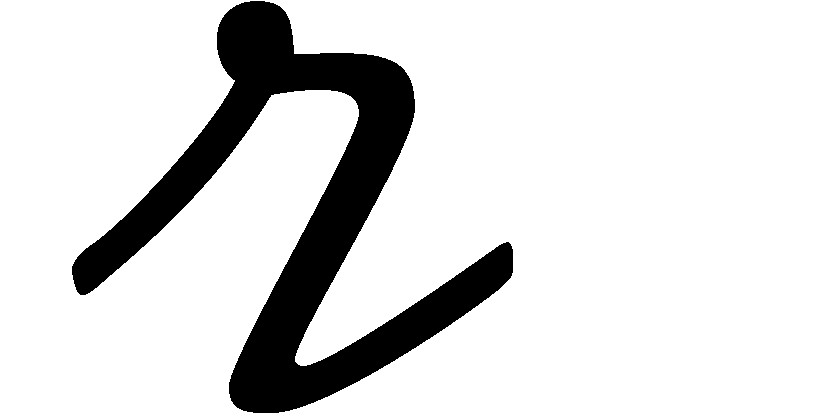
\includegraphics[trim= 1em 0 14em 0,clip]{ScriptR}}$}}}
\def\br{{\mbox{$\resizebox{.09in}{.08in}{
\includegraphics[trim= 1em 0 14em 0,clip]{BoldR}}$}}}


% title
\title{Electromagnetism}
\author{Richard Robinson}
\begin{document}
\maketitle
\setlength{\parindent}{0pt}

%-------------------------------------------

\chapter{Electricity}

\section{Electric Forces}
\textsc{In Electrodynamics}, there is typically a \emph{source point} $\b r '$ where a charge is located and a \emph{field point} $\b r$ where a field is calculated at. The \emph{seperation vector} is defined as
\begin{equation}
  \br \equiv \b r - \b r ' \qquad \hat\br = \br/\r
\end{equation}
upon definition of a coordinate system. Coulomb's law expresses the force of charges $q_i$ on another charge $q_0$, given by
\begin{equation}
    \b F \equiv K \sum \frac{q_0q_i}{\r^2} \hat\br = q_0 \b E
\end{equation}
When calculating the force via $E$, the charge density must be replaced by the respective equation. The charge differential is defined as
\begin{equation}
    dq \mapsto \lambda \, dx \sim \sigma \, dA \sim \rho \, dV
\end{equation}
When evaluating the results of the integration, the limiting cases such as $a \gg b$ can be found by evaluating the expression for $b = 0$.

\section{Electric Field}
The electric field at a point $P$ which acts like a positive test charge of a set of source charges is defined as
\begin{equation}
    \b E (\b r) \equiv K \sum \frac{q_i}{\r_i^2} \hat\br_i = K \int \frac{1}{\r ^2} \hat\br \; dq
\end{equation}
For most cases, symmetry can be utilized such that
\begin{equation}
    \b E = E_x \to \hat{\br} = \cos \theta
\end{equation}
An electric dipole describes the configuration of two opposite charges $q$ a distance $d$ apart. The electric dipole moment is defined as $p = qd$, which means the rate of the field for $x \gg d$ id $1/ \r ^3$.

\section{Energy}
The torque of an electric dipole is defined to be
\begin{equation}
    \tau = pE \sin \theta = \b p \times \b E
\end{equation}
assuming its direction is perpendicular to and into the page. The work done by the external field in turning a dipole is thus
\begin{equation}
    W = - \int_\theta \tau \; d \theta = pE(\Delta \cos \theta)
\end{equation}
which is related to the change in potential energy via
\begin{equation}
    U = - W = - \b p \cdot \b E
\end{equation}

\section{Gauss' Law}
Gauss' Law states the flux is the rate of change of an electric field of a Guassion surface; that is,
\begin{equation}
    \Phi_E = \oint \b E \cdot d \b A = q / \epsilon_0
\end{equation}
meaning for each infinitesimal point for a given surface, $\b E$ is in the direction of the filed lines, and $\b A$ is normal to the surface.

\bigskip
This results in $\Phi_E = 0$ if such closed surface does not enclose any charges and/or $\sum q = 0$. Because of this, $E$ can be calculated via \begin{equation}
    \sum EA = q / \epsilon_0 \qquad q \mapsto \lambda x \sim \sigma A
\end{equation}
For a conductor, the field $E = \sigma / \epsilon_0$.


\end{document}
